\title{The \textsc{ForSyDe-\LaTeX} utilities}
\author{
        George Ungureanu \\
                Department of Electronic Systems\\
        KTH---Royal Institute of Technology\\
        Stockholm, SWEDEN
}
\date{\today}

\documentclass[10pt]{article}
\usepackage[a4paper]{geometry}
\usepackage{forsyde-pc}
\usepackage[footnotesize]{caption}
\usepackage{longtable}
\usepackage{booktabs}
\usepackage{hyperref}
\usepackage{enumitem}
\usepackage{marginnote}
\usepackage{listings}
\pgfplotsset{compat=1.9}


\newenvironment{optionslist}[0]{ 
\begin{list}{}{
	\setlength{\itemindent}{-10pt}
%	\setlength{\topsep}{0pt}
	\setlength{\itemsep}{0pt}
	\setlength{\parsep}{0pt}
}}{\end{list}}
\newcommand\bookmark[1]{\marginpar{\ttfamily #1}}
\lstset{
  basicstyle=\footnotesize\ttfamily,
  % numbers=left,
  frame=single,
  numberstyle=\tiny\color{black!30},
  commentstyle=\color{blue}\textit,
  stringstyle=\color{magenta}\textit,
  flexiblecolumns=false,
  basewidth={0.5em,0.45em},
  breaklines=true,
  language={[LaTeX]TeX},
  texcsstyle=*\color{red}\bfseries,
  keywordstyle=\color{blue}\bfseries,
  morekeywords={tikzpicture,document},
  moretexcs={trans,standard,interface,basic,cluster,node,path,embed},
}
\def\opt#1{\color{gray}{#1}}
\def\man#1{\color{black}{#1}}

\begin{document}
\maketitle
\reversemarginpar

\begin{abstract}
This is the reference manual for the \LaTeX\ utilities used in the context of \textsc{ForSyDe}. All packages and their API features are documented here.
\end{abstract}

\section{Introduction}

This library was developed as an effort to standardize symbols and graphical primitives in documents related to \textsc{ForSyDe}, but also to provide tools and utilities for user convenience. \textsc{ForSyDe} is a high-level design methodology aiming at synthesizing correct-by-construction systems through formal means. For more information check \url{https://forsyde.ict.kth.se}.

The library contains the following main packages:
\begin{itemize}
\item \texttt{forsyde-tikz} : is a collection of \textsc{PGF} and
  \textsc{TikZ} styles, graphical primitives and commands for
  drawing \textsc{ForSyDe} process networks;
\item \texttt{forsyde-math} : is a collection of math symbols used in
  the \textsc{ForSyDe} formal notation. It is mainly focused on the
  ongoing \textsc{ForSyDe-Atom} methodology;
\item \texttt{forsyde-plot} : provides utilities for plotting
  \textsc{ForSyDe} signals;
\item \texttt{forsyde-legacy} : API for the previous versions of this
  library.
\end{itemize}

\section{Installation}

There are three main alternatives to use the libraries:

\begin{enumerate}
\item copy the contents of \texttt{forsyde-latex/src} under the \texttt{TEXMFHOME} path or any standard loading path, as specified by your \LaTeX\ compiler;
\item compile your document with the variable \texttt{TEXINPUTS} set to \texttt{/path/to/forsyde-latex/src/};
\item copy the contents of \texttt{forsyde-latex/src} in the same folder as your document and compile normally.
\end{enumerate}


\begin{figure}[htb]\centering
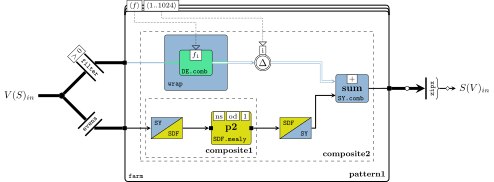
\includegraphics[width=\textwidth]{figs/example-forsyde-tikz}
\end{figure}

\lstinputlisting{figs/example-forsyde-tikz.tex}

\tableofcontents
\newpage

% A simple library for signal flow diagrams
% based on the pgf/tikz package of Till Tantau
%
% Author: Dr. Karlheinz Ochs, Ruhr-University of Bochum, Germany
% Version: 0.1
% Date: 2007/01/05
\NeedsTeXFormat{LaTeX2e}
\RequirePackage{pgfplots}
\RequirePackage{pgfkeys}
\RequirePackage{xparse}
\RequirePackage{todonotes} % WHA?!
\RequirePackage{ezkeys}
\usetikzlibrary{decorations.markings, shapes, calc, fit, backgrounds}

\ProvidesPackage{forsyde-tikz}
              [2014/12/01 v0.1 ForSyDe TikZ Library]

%
% Libraries for signal flow diagrams.
%
\usetikzlibrary{fsignals,fshapes,}


%%%%%%%%%%%%%
% CONSTANTS %
%%%%%%%%%%%%%
% Colors
\newcommand{\defaultdrawcolor}{black}     		% draw color of signal paths
\newcommand{\defaultfillcolor}{white}     		% draw color of signal paths
\definecolor{sycolor}{RGB}{148,183,215}
\definecolor{ctcolor}{RGB}{225,119,19}
\definecolor{decolor}{RGB}{80,229,154}
\definecolor{sdfcolor}{RGB}{220,220,20}
\definecolor{blackboxcolor}{gray}{0.80}
% line widths of
\newlength{\sepq}
\pgfmathsetlength{\sepq}{2pt}                % constant for small inter-node separation (used for example in function nodes)
\newcommand{\compositelinewidth}{.4pt}       % composite process line width
\newcommand{\skeletonlinewidth}{1pt}         % parallel processes line width
\newcommand{\signalpathlinewidth}{1pt}       % signal paths
\newcommand{\functionpathlinewidth}{.8pt}    % function paths
\newcommand{\vectorpathlinewidth}{4pt}       % vector paths
% sizes, etc.
\newcommand{\tokensize}{3.5pt}
\newcommand{\halftokensize}{1.75pt}
\newcommand{\vectorportsize}{3pt}
\newcommand{\signalportsize}{2pt}

%%%%%%%%%%%%%%%%%%%%%%%%
% GENERIC TIKZ HELPERS %
%%%%%%%%%%%%%%%%%%%%%%%%
% Positioning of node text.
% #1 = node label
% #2 = label text
\newcommand{\textaboveof}[2]{\pgftext[bottom,at=\pgfpointanchor{#1}{north},y=+1mm]{#2}}%
\newcommand{\textrightof}[2]{\pgftext[left,  at=\pgfpointanchor{#1}{east}, x=+1mm]{#2}}%
\newcommand{\textbelowof}[2]{\pgftext[top,   at=\pgfpointanchor{#1}{south},y=-1mm]{#2}}%
\newcommand{\textleftof} [2]{\pgftext[right, at=\pgfpointanchor{#1}{west}, x=-1mm]{#2}}%

\makeatletter
\newcounter{r}
\newcommand{\tikzgrid}{%
  \pgfsetxvec{\pgfpoint{\tikz@node@distance}{0mm}}%
  \pgfsetyvec{\pgfpoint{0mm}{\tikz@node@distance}}%
  \tikz@matrix%
}
\newcommand{\tikz@matrix}[1]{\tikz@@matrix#1@}%
\def\tikz@@matrix#1@{\do@rows#1\\@\\}%
\def\do@rows#1\\{%
  \ifx#1@%
  \else%
    \setcounter{r}{0}%
    \do@columns#1&@&%
    \pgftransformshift{\pgfpointxy{-\ther}{-1}}%
    \expandafter\do@rows%
  \fi}%
\def\do@columns#1&{%
  \if#1@%
  \else%
    \stepcounter{r}%
    \pgftransformshift{\pgfpointxy{1}{0}}%
    #1;%
    \expandafter\do@columns%
  \fi}%
\makeatother

%%%%%%%%%%%%%%%%
% ENVIRONMENTS %
%%%%%%%%%%%%%%%%
\newif\ifnolabel
\newif\ifnocolor
\pgfkeys{
	/tikz/nomoccolor/.is if=nocolor,
	/tikz/nomoclabel/.is if=nolabel,
	/tikz/type style/.store in = \typeStyle,
	/tikz/type style = \scriptsize\textit,
	/tikz/label style/.store in = \labelStyle,
	/tikz/label style = \textbf,
	/tikz/function style/.store in = \funcStyle,
	/tikz/function style = \scriptsize,
	/tikz/moc/.store in = \MoC,
	/tikz/moc = none,
	/tikz/mocin/.store in = \MoCin,
	/tikz/mocin = none,
	/tikz/mocout/.store in = \MoCout,
	/tikz/mocout = none,
}
\pgfkeys{
	/applicative/.is family, /applicative,
	default/.style = {moc=none, reverse = false, type= , ni=1, no=1, nf=0, f1=$ f_1 $, f2=$ f_2 $, f3=$ f_3 $, f4=$ f_4 $, line sep=0pt},
 	moc/.estore in = \pMoc,
 	type/.estore in = \pType,
	ni/.estore in = \pNIn,
	no/.estore in = \pNOut,
	nf/.estore in = \pNFunc,
	f1/.estore in = \pFuncA,
	f2/.estore in = \pFuncB,
	f3/.estore in = \pFuncC,
	f4/.estore in = \pFuncD,
	line sep/.estore in = \pLineSep,
	reverse/.is toggle,
}
\pgfkeys{
	/primitive/.is family, /primitive,
	default/.style = {moc=none, reverse = false, type= , ni=1, no=1,},
 	moc/.estore in = \pMoc,
 	type/.estore in = \pType,
	ni/.estore in = \pNIn,
	no/.estore in = \pNOut,
	reverse shape/.is toggle,
	reverse/.is toggle,
}
\pgfkeys{
	/interface/.is family, /interface,
	default/.style = {mocin = none, mocout = none, },
 	mocin/.estore in = \pMocIn,
 	mocout/.estore in = \pMocOut,
}
\newcommand{\getmoclabel}[1]{
	\ifthenelse{\equal{#1}{sy}}{SY}{
	\ifthenelse{\equal{#1}{de}}{DE}{
	\ifthenelse{\equal{#1}{ct}}{CT}{
	\ifthenelse{\equal{#1}{sdf}}{SDF}{}}}} 
}

%%%%%%%%%%%%%%%%%
% GENERIC NODES %
%%%%%%%%%%%%%%%%%

% Generic applicative leaf process
% #1 = environment keys
% #2 = node name
% #3 = node position
% #4 = node label
\newcommand{\applicative}[4][]{
	\pgfkeys{/applicative, default, #1}%
	\node[inner sep=0pt] (#2_label) at (#3) {\labelStyle{#4}};
	\node[func\pNFunc, font=\funcStyle, yshift=2\sepq+\pLineSep, anchor=south] (f#2) at (#2_label.north) {
		\ifnum \pNFunc>0 \nodepart{fa} \pFuncA\else\fi
		\ifnum \pNFunc>1 \nodepart{fb} \pFuncB\else\fi
		\ifnum \pNFunc>2 \nodepart{fc} \pFuncC\else\fi
		\ifnum \pNFunc>3 \nodepart{fd} \pFuncD\else\fi
	};
	\node[anchor=north, yshift=-\pLineSep] (#2_type) at (#2_label.south) {\typeStyle{\pType\ifnolabel\else\getmoclabel{\pMoc}\fi}};
	\iftoggle{/applicative/reverse}
		{\node[i\pNIn o\pNOut, rotate=180, inner sep=0pt, fit=(f#2)(#2_label)(#2_type),] (#2) {};}
		{\node[i\pNIn o\pNOut, inner sep=0pt, fit=(f#2)(#2_label)(#2_type),] (#2) {};}
	\begin{pgfonlayer}{background}
		\node[applshape, draw, moc=\pMoc, inner sep=0pt, fit=(f#2)(#2_label)(#2_type)] {};
	\end{pgfonlayer}
}


% Generic primite box-shaped leaf process
% #1 = environment keys
% #2 = node name
% #3 = node position
% #4 = node label
\newcommand{\primitivebox}[4][]{
	\applicative[#1, nf=0, line sep=-2pt]{#2}{#3}{#4}
}
% Generic primite special-shaped leaf process
% #1 = environment keys
% #2 = node name
% #3 = node position
\newcommand{\primitivespecial}[4][]{
	\pgfkeys{/primitive, default, #1}%
	\pgfmathsetlength{\foo}{max(\pNIn,\pNOut)*5pt}
	\iftoggle{/primitive/reverse shape}
		{\node[\pType, draw, moc=\pMoc, inner sep=\foo, rotate=180,] (#2_shape) at (#3) {};}	
		{\node[\pType, draw, moc=\pMoc, inner sep=\foo,] (#2_shape) at (#3) {};}	
	\iftoggle{/primitive/reverse}
		{\node[i\pNIn o\pNOut, rotate=180, inner sep=0pt, fit=(#2_shape),] (#2) {};}
		{\node[i\pNIn o\pNOut, inner sep=0pt, fit=(#2_shape),] (#2) {};}
}



\section{The \texttt{forsyde-legacy} package}
\label{sec:legacy-package}

This package offers an API for the legacy commands defined in older versions of the \ForSyDeLaTeX utilities. This way, documents compiled with old commands can be compiled with the newer versions of their respective library.

\subsection{\texttt{forsyde-tikz v0.3} or prior}
\label{sec:forsyde-tikz-v0.3}

Although from \texttt{v0.4} onward the draw commands have been heavily modified, the old commands could be mapped to the new API.

\begin{lstlisting}
\primitive[keys]         {id}{pos}{label}
\primitiven[keys]        {id}{pos}{label}
\leafstd[keys]           {id}{pos}{label}
\leafcustom[keys]        {id}{pos}
\compositestd[keys]      {id}{clustered nodes}{label}
\compositebbox[keys]     {id}{pos}{label}
\patterncluster[keys]    {id}{clustered nodes}{label}
\patternnodestd[keys]    {id}{pos}
\patternnodecustom[keys] {id}{pos}
\end{lstlisting}

\subsection{\texttt{forsyde-pc v0.3} or prior}
\label{sec:forsyde-pc-v0.3}

This package is obsolete and used to hold helpers associated to some \ForSyDe process constructors.

\begin{lstlisting}
\delay    [moc=,f1=,inner sep=,reverse]        {id}{pos}{label}
\delayn   [moc=,f1=,f2=,inner sep=,reverse]    {id}{pos}{label}
\map      [moc=,f1=,inner sep=,reverse]        {id}{pos}{label}
\comb     [moc=,f1=,inner sep=,reverse]        {id}{pos}{label}
\combII   [moc=,f1=,inner sep=,reverse]        {id}{pos}{label}
\combIII  [moc=,f1=,inner sep=,reverse]        {id}{pos}{label}
\combIV   [moc=,f1=,inner sep=,reverse]        {id}{pos}{label}
\scanl    [moc=,f1=,f2=,inner sep=,reverse]    {id}{pos}{label}
\scanlII  [moc=,f1=,f2=,inner sep=,reverse]    {id}{pos}{label}
\scanlIII [moc=,f1=,f2=,inner sep=,reverse]    {id}{pos}{label}
\scanld   [moc=,f1=,f2=,f3=,inner sep=,reverse]{id}{pos}{label}
\scanldII [moc=,f1=,f2=,f3=,inner sep=,reverse]{id}{pos}{label}
\scanldIII[moc=,f1=,f2=,f3=,inner sep=,reverse]{id}{pos}{label}
\moore    [moc=,f1=,f2=,f3=,inner sep=,reverse]{id}{pos}{label}
\mooreII  [moc=,f1=,f2=,f3=,inner sep=,reverse]{id}{pos}{label}
\mooreIII [moc=,f1=,f2=,f3=,inner sep=,reverse]{id}{pos}{label}
\mealy    [moc=,f1=,f2=,f3=,inner sep=,reverse]{id}{pos}{label}
\mealyII  [moc=,f1=,f2=,f3=,inner sep=,reverse]{id}{pos}{label}
\mealyIII [moc=,f1=,f2=,f3=,inner sep=,reverse]{id}{pos}{label}
\source   [moc=,f1=,f2=,inner sep=,reverse]    {id}{pos}{label}
\filter   [moc=,f1=,f2=,inner sep=,reverse]    {id}{pos}{label}
\hold     [moc=,f1=,inner sep=,reverse]        {id}{pos}{label}
\fillS    [moc=,f1=,f2=,inner sep=,reverse]    {id}{pos}{label}

\zip     [moc=,reverse]{id}{pos}
\zipIII  [moc=,reverse]{id}{pos}
\zipIV   [moc=,reverse]{id}{pos}
\zipV    [moc=,reverse]{id}{pos}
\zipVI   [moc=,reverse]{id}{pos}
\unzip   [moc=,reverse]{id}{pos}
\unzipIII[moc=,reverse]{id}{pos}
\unzipIV [moc=,reverse]{id}{pos}
\unzipV  [moc=,reverse]{id}{pos}
\unzipVI [moc=,reverse]{id}{pos}

\domaininterface[moc=,reverse]          {id}{pos}
\mocinterface   [mocin=,mocout=,reverse]{id}{pos}

\composite[ni=,no=,inner xsep=,inner ysep=,reverse] {id}{included}{label}
\blackbox [ni=,no=,inner xsep=,inner ysep=,reverse] {id}{included}{label}

\farm     [ni=,no=,inner xsep=,inner ysep=,reverse]                {id}{included}{label}
\farmI    [ni=,no=,f1=,inner xsep=,inner ysep=,reverse]            {id}{included}{label}
\farmII   [ni=,no=,f1=,f2=,inner xsep=,inner ysep=,reverse]        {id}{included}{label}
\farmIII  [ni=,no=,f1=,f2=,f3=,inner xsep=,inner ysep=,reverse]    {id}{included}{label}
\farmIV   [ni=,no=,f1=,f2=,f3=,f4=,inner xsep=,inner ysep=,reverse]{id}{included}{label}
\pipe     [ni=,no=,inner xsep=,inner ysep=,reverse]                {id}{included}{label}
\pipeI    [ni=,no=,f1=,inner xsep=,inner ysep=,reverse]            {id}{included}{label}
\pipeII   [ni=,no=,f1=,f2=,inner xsep=,inner ysep=,reverse]        {id}{included}{label}
\pipeIII  [ni=,no=,f1=,f2=,f3=,inner xsep=,inner ysep=,reverse]    {id}{included}{label}
\pipeIV   [ni=,no=,f1=,f2=,f3=,f4=,inner xsep=,inner ysep=,reverse]{id}{included}{label}
\reduce   [ni=,no=,inner xsep=,inner ysep=,reverse]                {id}{included}{label}
\reduceI  [ni=,no=,f1=,inner xsep=,inner ysep=,reverse]            {id}{included}{label}
\reduceII [ni=,no=,f1=,f2=,inner xsep=,inner ysep=,reverse]        {id}{included}{label}
\reduceIII[ni=,no=,f1=,f2=,f3=,inner xsep=,inner ysep=,reverse]    {id}{included}{label}
\reduceIV [ni=,no=,f1=,f2=,f3=,f4=,inner xsep=,inner ysep=,reverse]{id}{included}{label}

\unzipx     [reverse]         {id}{position}
\zipx       [reverse]         {id}{position}
\unzipv     [reverse]         {id}{position}
\zipv       [reverse]         {id}{position}
\splitatv   [f1=,reverse]     {id}{position}
\catv       [reverse]         {id}{position}
\oddsv      [reverse]         {id}{position}
\evensv     [reverse]         {id}{position}
\reversev   [reverse]         {id}{position}
\groupv     [reverse]         {id}{position}
\concatv    [reverse]         {id}{position}
\filteridxv [f1=,reverse]     {id}{position}
\gatherv    [f1=,f2=,reverse] {id}{position}
\gatherAdpv [f1=,f2=,reverse] {id}{position}
\selectv    [reverse]         {id}{position}
\distributev[f1=,reverse]     {id}{position}
\filterv    [f1=,reverse]     {id}{position}
\getv       [f1=,reverse]     {id}{position}

\visualoddsv   [reverse]{id}{pos}
\visualevensv  [reverse]{id}{pos}
\visualreversev[reverse]{id}{pos}
\visualgroupv  [reverse]{id}{pos}
\visualconcatv [reverse]{id}{pos}
\end{lstlisting}


%%% Local Variables:
%%% TeX-command-default: "Make"
%%% mode: latex
%%% TeX-master: "../refman"
%%% End:



% \section{The \texttt{forsyde-pc} package}

% The \texttt{forsyde-pc} package includes \textsc{ForSyDe} process constructors, written as macros. For a detailed theoretical background in process constructors check the \textsc{ForSyDe} homepage. It is included with: 

% \begin{verbatim}
% 	\usepackage{forsyde-pc}
% \end{verbatim}

% Following is a list with all process constructors including valid option keys:

% \begin{lstlisting}
% \delay    [moc=,f1=,inner sep=,reverse]        {id}{pos}{label}
% \delayn   [moc=,f1=,f2=,inner sep=,reverse]    {id}{pos}{label}
% \map      [moc=,f1=,inner sep=,reverse]        {id}{pos}{label}
% \comb     [moc=,f1=,inner sep=,reverse]        {id}{pos}{label}
% \combII   [moc=,f1=,inner sep=,reverse]        {id}{pos}{label}
% \combIII  [moc=,f1=,inner sep=,reverse]        {id}{pos}{label}
% \combIV   [moc=,f1=,inner sep=,reverse]        {id}{pos}{label}
% \scanl    [moc=,f1=,f2=,inner sep=,reverse]    {id}{pos}{label}
% \scanlII  [moc=,f1=,f2=,inner sep=,reverse]    {id}{pos}{label}
% \scanlIII [moc=,f1=,f2=,inner sep=,reverse]    {id}{pos}{label}
% \scanld   [moc=,f1=,f2=,f3=,inner sep=,reverse]{id}{pos}{label}
% \scanldII [moc=,f1=,f2=,f3=,inner sep=,reverse]{id}{pos}{label}
% \scanldIII[moc=,f1=,f2=,f3=,inner sep=,reverse]{id}{pos}{label}
% \moore    [moc=,f1=,f2=,f3=,inner sep=,reverse]{id}{pos}{label}
% \mooreII  [moc=,f1=,f2=,f3=,inner sep=,reverse]{id}{pos}{label}
% \mooreIII [moc=,f1=,f2=,f3=,inner sep=,reverse]{id}{pos}{label}
% \mealy    [moc=,f1=,f2=,f3=,inner sep=,reverse]{id}{pos}{label}
% \mealyII  [moc=,f1=,f2=,f3=,inner sep=,reverse]{id}{pos}{label}
% \mealyIII [moc=,f1=,f2=,f3=,inner sep=,reverse]{id}{pos}{label}
% \source   [moc=,f1=,f2=,inner sep=,reverse]    {id}{pos}{label}
% \filter   [moc=,f1=,f2=,inner sep=,reverse]    {id}{pos}{label}
% \hold     [moc=,f1=,inner sep=,reverse]        {id}{pos}{label}
% \fillS    [moc=,f1=,f2=,inner sep=,reverse]    {id}{pos}{label}

% \zip     [moc=,reverse]{id}{pos}
% \zipIII  [moc=,reverse]{id}{pos}
% \zipIV   [moc=,reverse]{id}{pos}
% \zipV    [moc=,reverse]{id}{pos}
% \zipVI   [moc=,reverse]{id}{pos}
% \unzip   [moc=,reverse]{id}{pos}
% \unzipIII[moc=,reverse]{id}{pos}
% \unzipIV [moc=,reverse]{id}{pos}
% \unzipV  [moc=,reverse]{id}{pos}
% \unzipVI [moc=,reverse]{id}{pos}

% \domaininterface[moc=,reverse]          {id}{pos}
% \mocinterface   [mocin=,mocout=,reverse]{id}{pos}

% \composite[ni=,no=,inner xsep=,inner ysep=,reverse] {id}{included}{label}
% \blackbox [ni=,no=,inner xsep=,inner ysep=,reverse] {id}{included}{label}

% \farm     [ni=,no=,inner xsep=,inner ysep=,reverse]                {id}{included}{label}
% \farmI    [ni=,no=,f1=,inner xsep=,inner ysep=,reverse]            {id}{included}{label}
% \farmII   [ni=,no=,f1=,f2=,inner xsep=,inner ysep=,reverse]        {id}{included}{label}
% \farmIII  [ni=,no=,f1=,f2=,f3=,inner xsep=,inner ysep=,reverse]    {id}{included}{label}
% \farmIV   [ni=,no=,f1=,f2=,f3=,f4=,inner xsep=,inner ysep=,reverse]{id}{included}{label}
% \pipe     [ni=,no=,inner xsep=,inner ysep=,reverse]                {id}{included}{label}
% \pipeI    [ni=,no=,f1=,inner xsep=,inner ysep=,reverse]            {id}{included}{label}
% \pipeII   [ni=,no=,f1=,f2=,inner xsep=,inner ysep=,reverse]        {id}{included}{label}
% \pipeIII  [ni=,no=,f1=,f2=,f3=,inner xsep=,inner ysep=,reverse]    {id}{included}{label}
% \pipeIV   [ni=,no=,f1=,f2=,f3=,f4=,inner xsep=,inner ysep=,reverse]{id}{included}{label}
% \reduce   [ni=,no=,inner xsep=,inner ysep=,reverse]                {id}{included}{label}
% \reduceI  [ni=,no=,f1=,inner xsep=,inner ysep=,reverse]            {id}{included}{label}
% \reduceII [ni=,no=,f1=,f2=,inner xsep=,inner ysep=,reverse]        {id}{included}{label}
% \reduceIII[ni=,no=,f1=,f2=,f3=,inner xsep=,inner ysep=,reverse]    {id}{included}{label}
% \reduceIV [ni=,no=,f1=,f2=,f3=,f4=,inner xsep=,inner ysep=,reverse]{id}{included}{label}

% \unzipx     [reverse]         {id}{position}
% \zipx       [reverse]         {id}{position}
% \unzipv     [reverse]         {id}{position}
% \zipv       [reverse]         {id}{position}
% \splitatv   [f1=,reverse]     {id}{position}
% \catv       [reverse]         {id}{position}
% \oddsv      [reverse]         {id}{position}
% \evensv     [reverse]         {id}{position}
% \reversev   [reverse]         {id}{position}
% \groupv     [reverse]         {id}{position}
% \concatv    [reverse]         {id}{position}
% \filteridxv [f1=,reverse]     {id}{position}
% \gatherv    [f1=,f2=,reverse] {id}{position}
% \gatherAdpv [f1=,f2=,reverse] {id}{position}
% \selectv    [reverse]         {id}{position}
% \distributev[f1=,reverse]     {id}{position}
% \filterv    [f1=,reverse]     {id}{position}
% \getv       [f1=,reverse]     {id}{position}

% \visualoddsv   [reverse]{id}{pos}
% \visualevensv  [reverse]{id}{pos}
% \visualreversev[reverse]{id}{pos}
% \visualgroupv  [reverse]{id}{pos}
% \visualconcatv [reverse]{id}{pos}
% \end{lstlisting}

% \newpage
% \section
% \section{PGF nodes} \label{section_shapes}

% All graphical elements in the \texttt{forsyde-tikz} package are created using custom PGF shapes defined in \texttt{tikzlibraryfshapes.code.tex}. You can create new elements by combining them, as can be seen in \texttt{tikzlibraryforsyde.code.tex}. Following is a list with these shapes:

% \begin{optionslist}
% \item \texttt{ports e[0..10]o[0..10]} : defines anchors for the input/output pwrts.
% \item \texttt{func[0..4]} : defines boxes and anchors for the functions nodes.
% \item \texttt{leaf shape} : the shape of a standard leaf process outer box.
% \item \texttt{zip shape} : the shape of a custom zip process.
% \item \texttt{interface shape 0} : the node shape of an interface process.
% \item \texttt{interface shape 180} : the node shape of a reversed interface process.
% \item \texttt{comp shape} : the shape of a composite process.
% \item \texttt{dp shape} : the shape of a data-parallel pattern.
% \item \texttt{pipe shape} : the shape of a time-parallel (pipelined) pattern.
% \item \texttt{merge shape} : the shape of a merging (e.g. reduce) pattern.
% \item \texttt{custom conduit i[2..8]o[2..8]} : the inner node depicting the conduit in a custom (visual) transition pattern.
% \item \texttt{trans shape v[1..8]v[1..8]} : the outer box of a transition pattern, depicting vector(s) on one side and vector(s) on the other side.
% \item \texttt{trans shape s1v1} : the outer box of a transition pattern, depicting a signal on one side and a vector on the other side.
% \item \texttt{trans shape v1gv1} : the outer box of a transition pattern, depicting a vector on one side and a group of vectors on the other side.
% \end{optionslist}


% \begin{tikzpicture}[]
% \newleaf[]{lc}{0,0}{hallo};  
% \newleaf[ni=2, anchor=north]{l1}{2,0}{hallo1};
% \basic[shape=primitive,nf=1] {u} {3,0} {q};
% \end{tikzpicture}


\end{document}
%%% Local Variables:
%%% TeX-command-default: "Make"
%%% mode: latex
%%% TeX-master: t
%%% End:
